\chapterimage{./Pictures/cover-gear} % Chapter heading image
\chapter{TP5+TP6 : Hiérarchie de processus, signaux}

\section{Gestion des signaux : envoi et reception}

\subsection{Exercice 1 : Droits et signaux}

\inputminted[linenos]{cpp}{../sources/cpp/TP5-6/ex1.c}

\subsection{Exercice 2 : capture de signal et traduction en langage C}

\inputminted{bash}{../sources/cpp/TP5-6/ex2-boucle.sh}
Et maintenant en langage \texttt{C} :
\inputminted[linenos,firstline=5, lastline=27]{cpp}{../sources/cpp/TP5-6/ex2.c}

\subsection{Exercice 3 : Capture de signaux et redirections (exercice difficile)}

\inputminted[linenos]{bash}{../sources/cpp/TP5-6/ex3-testKillerSignal.sh}

\subsection{Exercice 4 : envoi multiples et capture de signal en C}

\inputminted{bash}{../sources/cpp/TP5-6/ex4-captureShell.sh}
Et maintenant en langage \texttt{C} :
\inputminted[linenos,firstline=5, lastline=23]{cpp}{../sources/cpp/TP5-6/ex4.c}

\section{Gestion des processus}

\subsection{Exercice 5 : Processus en premier-plan / Arriere-plan}

\subsection{Exercice 6 : Duplication et recouvrement de processus}

\section{Gestion des processus - Suite}

\subsection{Exercice 7 : Duplication de processus}

\subsection{Exercice 8 : Creation et destruction de processus}

\subsection{Exercice 9 : Evaluation du nombre de processus}
\inputminted[linenos,firstline=5, lastline=9]{cpp}{../sources/cpp/TP5-6/ex9-programme1.c}
\begin{figure}[H]
\centering
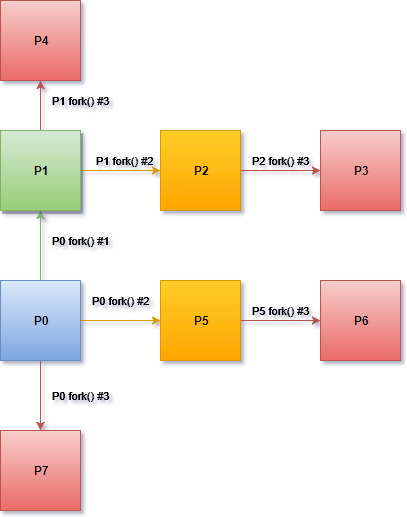
\includegraphics[width=200pt]{./cpp/Pictures/tp5+tp6-ex9-programme1}
\caption{Duplication de processus 1}
\label{Duplication de processus 1}
\end{figure}

\inputminted[linenos,firstline=5, lastline=9]{cpp}{../sources/cpp/TP5-6/ex9-programme2.c}
\begin{figure}[H]
\centering
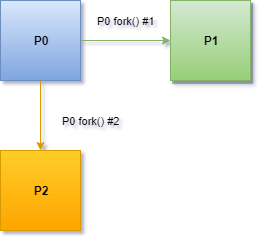
\includegraphics[width=200pt]{./cpp/Pictures/tp5+tp6-ex9-programme2}
\caption{Duplication de processus 2}
\label{Duplication de processus 2}
\end{figure}

\inputminted[linenos,firstline=5, lastline=13]{cpp}{../sources/cpp/TP5-6/ex9-programme3.c}
\begin{figure}[H]
\centering
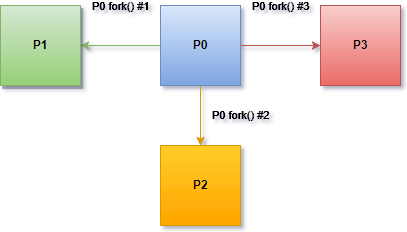
\includegraphics[width=200pt]{./cpp/Pictures/tp5+tp6-ex9-programme3}
\caption{Duplication de processus 3}
\label{Duplication de processus 3}
\end{figure}

\subsection{Exercice 10 : Conjonctions, Disjonctions, et Duplication}

\inputminted[linenos,firstline=5, lastline=8]{cpp}{../sources/cpp/TP5-6/ex10-conjonction1.c}
\begin{figure}[H]
\centering
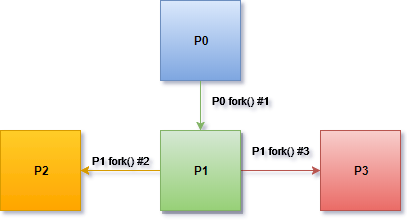
\includegraphics[width=200pt]{./cpp/Pictures/tp5+tp6-ex10-conjonction1}
\caption{Conjonction de processus 1}
\label{Conjonction de processus 1}
\end{figure}

\inputminted[linenos,firstline=5, lastline=8]{cpp}{../sources/cpp/TP5-6/ex10-conjonction2.c}
\begin{figure}[H]
\centering
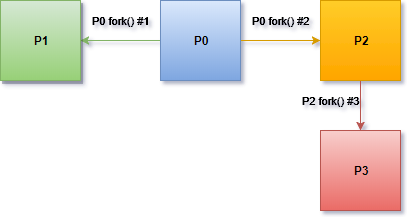
\includegraphics[width=200pt]{./cpp/Pictures/tp5+tp6-ex10-conjonction2}
\caption{Conjonction de processus 2}
\label{Conjonction de processus 2}
\end{figure}

\subsection{Exercice 11 : Terminaison normale de processus}
\inputminted[linenos,firstline=5, lastline=11]{cpp}{../sources/cpp/TP5-6/ex11-programme1.c}
\inputminted[linenos,firstline=5, lastline=14]{cpp}{../sources/cpp/TP5-6/ex11-programme2.c}
\inputminted[linenos,firstline=5, lastline=19]{cpp}{../sources/cpp/TP5-6/ex11-programme3.c}
